\documentclass[14pt,a4paper]{extreport}
%\usepackage[utf8]{inputenc}
\usepackage{amsmath}
\usepackage{amsfonts}
\usepackage{amssymb}
\usepackage{mathptmx}
\usepackage{fullpage}
\usepackage{graphicx}


%\usepackage{setspace}  
%\setstretch{1.5}
\usepackage{cite}
\usepackage[left=3.5cm,right=2cm,top=3cm,bottom=3.5cm]{geometry}


\author{Ngo Thanh Vu}
\title{EXPLORATION  OF  RIA  TECHNOLOGIES  AND  DEVELOPMENT  OF  A  WEB-BASED DIAGRAMMING TOOL}
%\linespread{1.5}
\begin{document}
\maketitle
\tableofcontents
\listoffigures
\listoftables


%Acknowledgement
\begin{titlepage}
\textbf{Acknowledgement}

I dedicate special gratefulness to my instructor, Dr.Do Lenh Hung Son for guiding and assisting me during the time i was working with him. I would like to thank all members in the Advanced Program of Computer Sciences including my classmates, seniors, professors, and all members in the Teaching Staff of Faculty of Information Technology and Academic Affairs. They play a very important part to the success of my thesis
\end{titlepage}

%Abstract
\begin{titlepage}
\textbf{Abstract}

Since 1999, when the term "Web 2.0" was introduced , which is associated with a richer web facilitating social media, user-generated content as well as interaction and collaboration, business applications have become increasingly web-oriented . While the web in its roots was limited to passive viewing of content created by others, it has moved towards an application platform for desktop-like applications within the last decade. Utilizing these advantages, in this thesis, I present a web application to design diagrams which can be considered as a Rich Internet Application (RIA) and Single Page Application (SPA). I also took a survey to explore and choose state of the art technologies which support to build such web application.I demonstrated by building an web application using the chosen technologies and integrating them . I also introducing about RIA and SPA as well as HTML5, CSS3, AngularJS (Javascript Framework), GoJS (Diagram Library), and other technologies i have been using for this application.

\end{titlepage}

\chapter{INTRODUCTION}

Nowadays Internet is increasing its popularity dramatically, people tend to work online with web browsers more than ever\cite{survey,Gvu,Center} . A survey in early 2010 \cite{Internet} showed that 74\% of American adults and 93\% of teenagers of age 12-17 use the Internet. More specific, email and search engines are the two most popular services that people do online\cite{Online}. Web browsers play a key role of being a door to link users to an enormous source of information: websites. Therefore, The popularity of web browser is premise for the emerging of web applications which uses web browser as a client. The ability to update and maintain web applications without distributing and installing software on potentially thousands of client computers is a key reason for their popularity, as is the inherent support for cross-platform compatibility\cite{WebApp}.
\\

Low-level JavaScript libraries like jQuery\footnote{http://jquery.com/}, Prototype\footnote{http://www.prototypejs.org/}, Underscore.js\footnote{http://documentcloud.github.com/underscore/}, etc., provide a convenient API for manipulating the Document Object Model (DOM) in a uniform way across different browser implementations. However no means to structure
the application code are provided, usually resulting in lots of DOM element selector and callback code\cite{Real}. This "spaghetti code of the 21st century" \cite{MT08} is reminiscent of software development in the 1970s and leads to poor maintainability of applications. That’s where web application frame-works come into play. Besides disburden developers from writing boilerplate code, frameworks can structure web applications enforcing the separation of different application parts. According to the Model-View-Controller design pattern \cite{Ree79b, Ree79a} frameworks usually separate user interface definition, application data, and business logic. Due to this modularization, frameworks support the fast development of applications and promote reuse as well as maintainability. As of today, several frameworks are available.
\\

The extensive usage of JavaScript in today 's web application induces the need for frameworks supporting faster development, better reusability and maintainability. As Model-View-Controller(MVC)is a well-known design pattern for server-side application development. It becomes even more important on client-side leading to several prevalent JavaScript MVC frameworks\cite{Real}. Therefore client-side JavaScript application frameworks will be of great importance for the development of futer web-based business application.
\\

The goal of this thesis is to analyze existing JavaScript frameworks with respect to various criteria such as structure, data-biding, Testing ability,ect. From the set of reviewed frameworks, one should be selected to design and implement a web application for edit and design interactive diagrams. Besides, JavaScript libraries supporting implementing interactive diagrams are also analyzed and selected. Other selected technologies for front-end development and database are also integrated. This thesis proposes a way of survey and select  as well as integrating state of the art technologies into a web application.In fact, there are web applications supporting edit interactive diagrams. I can list several famous name as follow. Big guy Google's draw.io\footnote{https://www.draw.io} has his own online diagram drawing application which use MxGraph\footnote{www.jgraph.com/mxgraph.html‎} and his own cloud storage to implement. Creately\footnote{http://http://creately.com/} provide an environment for designing diagrams with support of collaboration implemented with Adobe Flash\footnote{http://www.adobe.com/software/flash/about/}. Gliffy\footnote{http://www.gliffy.com/} and Lucidchart\footnote{https://www.lucidchart.com/} are also famous for their beautiful diagrams with collaboration support. Although the features demonstrated cannot be fancy and various as in those example application , This thesis is still an evidence of using JavaScript frameworks and cloud storage actually makes web application development less complex, less cumbersome and more maintainable than in the past.
\\
\\
\\

Concretely, This thesis contains
\begin{enumerate}
\item Conducting surveys about JavaScript frameworks and JavaScript Libraries which support implementing 
\item Exploration of selected technologies
\item Implementing a web application using selected technologies
\item Evaluation about the advantages that those technologies brought as well as some future works remain to be done
\end{enumerate}
This thesis consists of six chapters. Below is each chapter’s preview:
\begin{list}{•}{•}

\item  Chapter 1- Introduction. A brief introduction about the trend of web application as well as the importance JavaScript frameworks in web application development, their advantages and briefly describe what i do.

\item Chapter 2 - Technology survey. A brief introduction about RIA and SPA. I present surveys about JavaScript frameworks and JavaScript graph libraries, Their result and reasons why i choose them

\item Chapter 3 - Exploration of key technologies. Describe in details about AngularJS, GoJS, Mongolab, Angular Boostrap, Jquery, Semantic-UI, their advantages and reasons for choosing them.

\item Chapter 4 - Building application using selected technologies. Describe in details how i implemented using selected technologies.

\item Chapter 5 - Discussion \& conclusion. I present further disscussion about the web application, pros and cons, vision for future works. i end the thesis by summing up what i have done.

\end{list}

\chapter{TECHNOLOGY SURVEY }
	\textsl{In this chapter, the concept of Rich Internet Application(RIA) and Single Page Application(SPA) is introduced. Besides, I need to define some criteria based on what Javascript framework can bring. Consequently, i conducted surveys about JavaScript frameworks and JavaScript Graph libraries in order to support the web application development}
	\newpage 

	\section{RIA and SPA }
		\subsection{Introduction}
	

	
		Since 1990, when the first web browser prototype called "WorldWideWeb"\cite{BL12} was released by Tim Berners-Lee, the web has evolved from a simple document sharing system to a multimedia content distribution and application runtime environment. The major evolution step which is depicted in the picture below. At first, web pages were simple documents contain nothing but text and images.Users could navigate between different pages by hyperlinks.\\\\
		
		 At that time the capability of the web was limited. Due to emerging software development capabilities, the web was used increasingly as application platform in the second period. This is the time when the term \textbf{single-page application} also known as \textbf{single-page interface (SPI)} appears. It is a web application or web site that fits on a single web page with the goal of providing a more fluid user experience akin to a desktop application.
		 
		\begin{figure}[ht]
		 \begin{center}
			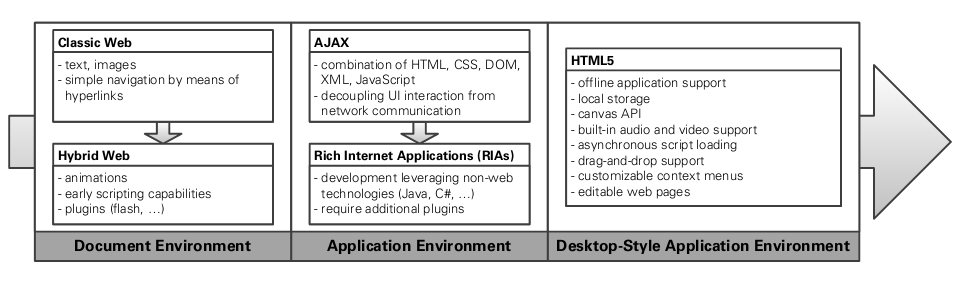
\includegraphics[scale=0.5]{WebEvolve.png}
			\caption{Major evolution steps of the Web\cite{TM11}}
		\end{center}
		\end{figure}

		
		\textbf{Asynchronous JavaScript and XML (AJAX)}, introduced by Jesse James Garret in 2005\cite{Gar05} ,changed the primary interaction model of the web and therefore increased its use as an application environment. However, the browser at this time was not supplied enough comprehensive sets of \textbf{API} and complex graphic capabilities.To provide such sets of APIs which were similar to the desktop application, \textbf{RIA} is introduced. It is a Web application that has many of the characteristics of desktop application software, Users generally need to install a software framework using the computer's operating system before launching the application, which typically downloads, updates, verifies and executes the RIA\cite{RIA} .Examples for RIA
platforms are Adobe Flash,Java FX and Microsoft Silverlight.
		
		
		\subsection{The current approaches}
		
			\subsubsection{JavaScript}
		
		 Currently JavaScript is the predominant implementation technique for plug-in free applications in the web. JavaScript applications can be built by means of pure JavaScript, leveraging low-level libraries like jQuery or high-level frameworks like Knockout.js. Since applications built by means of JavaScript use standardized web technologies, they do not require a dedicated plug-in
as runtime environment.
			\subsubsection{Non-JavaScript}
		
			Non JavaScript, but plug-in based applications require the installation of additional browser plug-ins serving as runtime aaenvironment. Example technologies belonging to this category are Adobe Flash , Java FX and Microsoft Silverlight.Some non JavaScript, but plug-in free implementation techniques are available too. Some of them enable the developer to write the application’s code in a language abstracting from concrete web technologies like HTML, CSS, etc. Two example technologies are Google Web Toolkit enabling web application development in Java, and CoffeeScript.
		
	\section{JavaScript Framework Selection}
		\subsection{Overviews of some JavaScript frameworks}
		\subsubsection{JavaScript Library view}
			we may define this group consists of the JavaScript framework which slots into your existing architecture and add specific functionality. Example to this kind are \textbf{Knockout.js, JQuery, JQueryUI}.JavaScript widget libraries such as \textbf{Ext JS , DHTMLX , Dojo Toolkit} were developed, allowing for developers to concentrate more upon more distinctive applications of Ajax.
		\subsubsection{JavaScript Framework view}
			This kind of framework gives you an architecture (file structure, etc.) that you are meant to follow and, if you do, are intended to handle all common requirements. Some example are \textbf{Ember.js , Angular.js , YUI, Backbone.js}
		
		\subsection{Framework Selection Characteristics}
		These are some criteria for choosing the framework
		\begin{itemize}
			\item The license under which the framework is released
			\item The size of the framework
			\item Community: the number of users or posts in the forum they use or on GitHub( Jan 2013) indicating the community support, as well as the website of the framework usually providing tutorials and a more or less comprehensive documentation.
			\item Programming language
			\item Js include indicates whether we need to include a js file into the website or not
			\item Basic UI component support: indicates that whether the framework provides their own basic component like text field, check box, combo box, form, date picker, ...
			\item Advanced UI widget library indicates that whether the framework support advanced components like grid view, tree, auto-complete, 
			
		\end{itemize}
		\subsection{Survey of Existing Frameworks}
		\subsubsection{Google Web Toolkit(GWT)}
			\begin{itemize}
				\item Overview: \textbf{GWT} provides an open source set of tools that allows web developers to create and maintain complex JavaScript front-end applications in Java. Besides,it supports writing both the client-side code and the server-side code in Java
				\item Pros: 
					\begin{itemize}
						\item supports ability to debug
						\item Strong community
						\item good documents,demos, samples
						\item supports lots of features
						\item No JavaScript syntax errors
						\item it's good for those who had java background and doesn't really appreciate the power of JavaScript (for both GWT and Vaadin
					\end{itemize}
				\item Cons:
					\begin{itemize}
						\item kind of a little too few stunning UI components comparing with Vaadin
						\item don't see much demo or support about drag drop
					\end{itemize}
			\end{itemize}
			\begin{figure}
				\begin{center}
					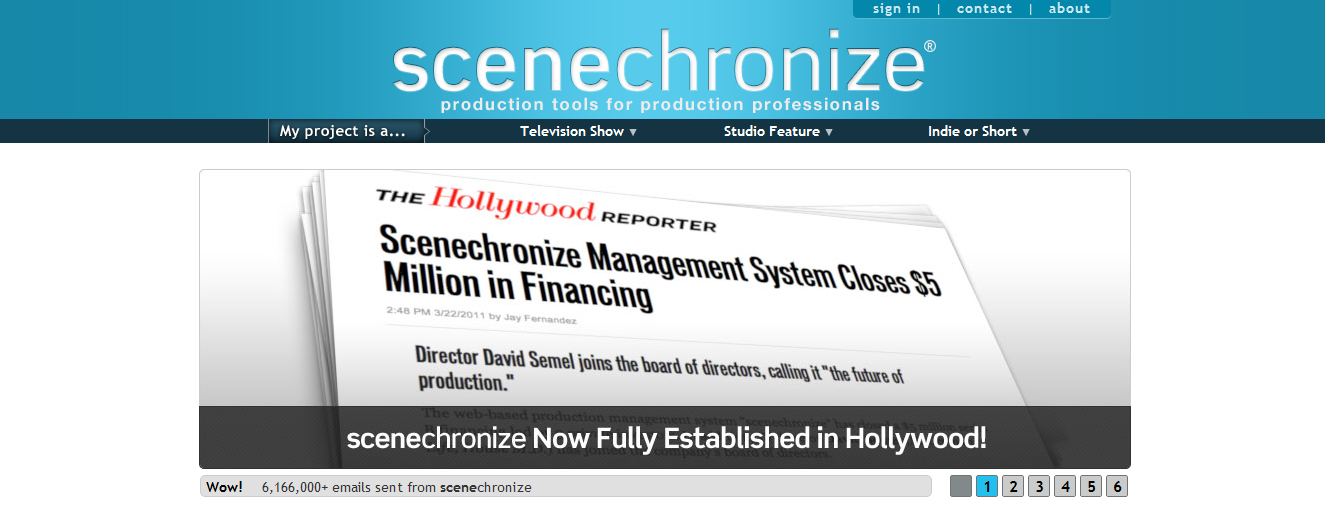
\includegraphics[scale=0.5]{GWT.png}
					\caption{ An example created by GWT}
				\end{center}
 			\end{figure}
			
		\subsubsection{Vaadin}
			\begin{itemize}
			\item Overview: features a server-side architecture and client-side is built on top of GWT.
				\item Pros: 
					\begin{itemize}
						\item Wide variety of UI components
						\item Drag and Drop for Tables, Panels and Trees components have real nice demos and tutorial
						\item Simple to learn, it has a book, a road map, a forum
						\item With Vaadin, you can build a nice app with almost a half of lines of code and still the application seems more complete compare with GWT
						
					\end{itemize}
				\item Cons:
					\begin{itemize}
						\item for advanced customization you'll need to write more in CSS, HTML, JavaScript
						\item Client side is not extensible and very chaotic
						\item html files is really heavy and takes long render time due to lots of components are added
						
					\end{itemize}
			\end{itemize}
			\begin{figure}
				\begin{center}
					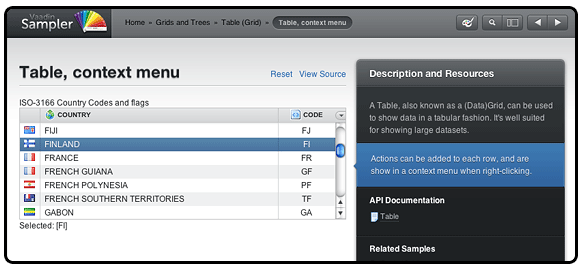
\includegraphics[scale=1.1]{Vaadin.png}
					\caption{An example created by Vaadin}
				\end{center}
			\end{figure}
		\subsubsection{SproutCore}
			\begin{itemize}
			\item Overview: an open-source framework for building blazingly fast, innovative user experiences on the web supported by Apple. It is also one of the largest frameworks.
				\item Pros: 
					\begin{itemize}
						\item MIT license
						\item Bindings support.
						\item Solid community. 
						\item Tons of features.
					
					\end{itemize}
				\item Cons:
					\begin{itemize}
						\item Overly prescriptive. 
						\item Hard to decouple from unneeded features.
						\item Forces a native-like paradigm
						
					\end{itemize}
			\end{itemize}
			\begin{figure}
				\begin{center}
				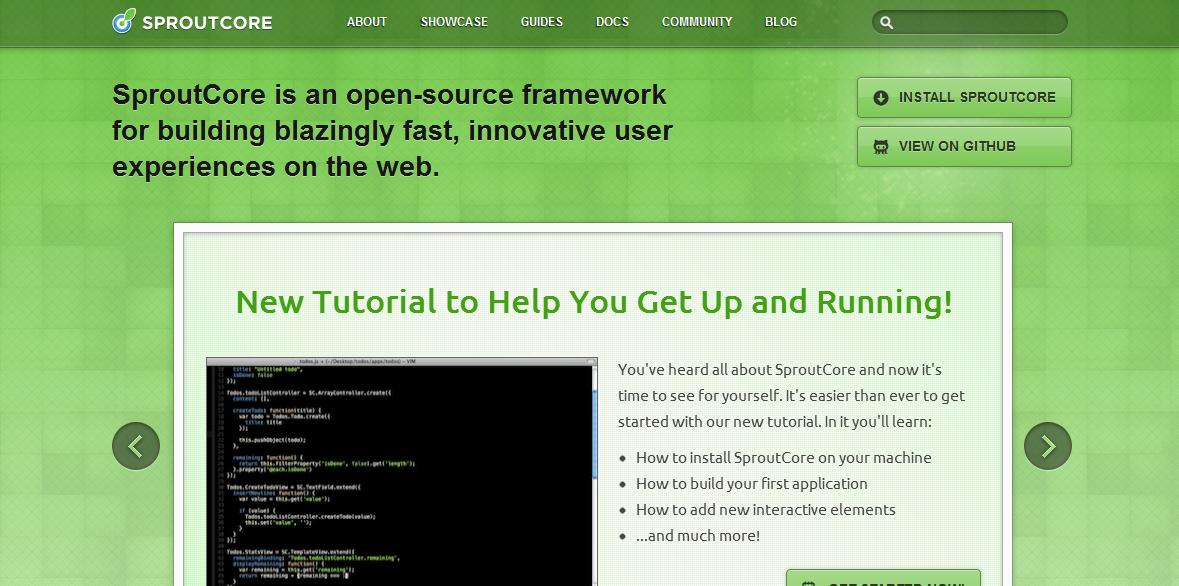
\includegraphics[scale=0.5]{Sproutcore.png}
				\caption{An example created by SproutCore}
				\end{center}
			
			\end{figure}

		\subsubsection{Dojo}
			\begin{itemize}
				\item Overview: DOJO is one of the leading JavaScript framework.
				\item Pros: 
					\begin{itemize}
						\item documents and tutorials in details
						\item  has all the components you would most likely use
					\end{itemize}
				\item Cons:
					\begin{itemize}
						\item API stability
						\item Demo is not very clear and scatter
						\item Many have commented that Dojo seems difficult to learn and get started with
			
					\end{itemize}
			\end{itemize}
			
			\begin{figure}
				\begin{center}
				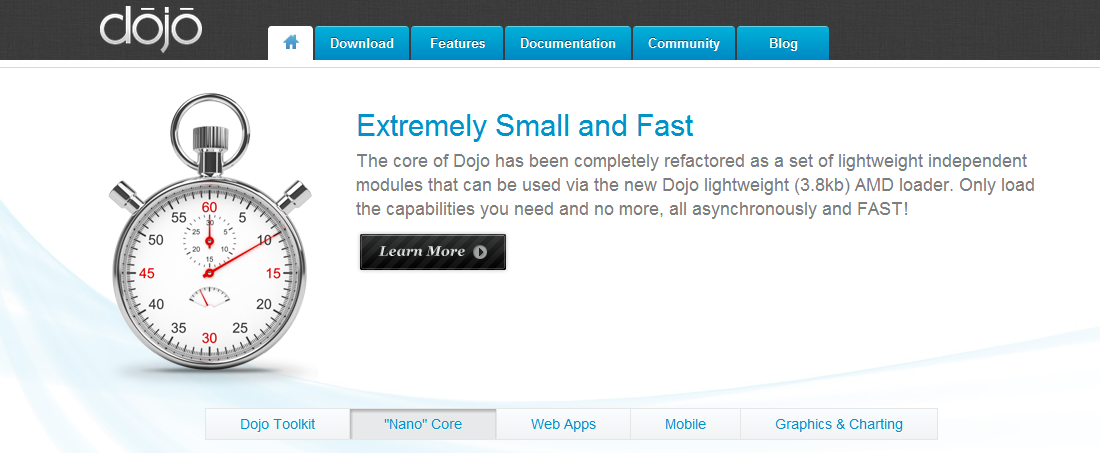
\includegraphics[scale=0.6]{Dojo.png}
				 \caption{An example created by Dojo}
				\end{center}			
			\end{figure}

		\subsubsection{JavaScriptMVC}
			\begin{itemize}
				\item Overview: an open-source framework containing the best ideas in jQuery development,a collection of the best practices and tools for building JavaScript applications. Built on top of jQuery"
				\item Pros: 
					\begin{itemize}
						\item using Controllers can make a clean, tight code that is easy to find
						\item is very lightweight, it's jQuery based
						
					\end{itemize}
				\item Cons:
					\begin{itemize}
						\item No preset UI layer implementations
						
					\end{itemize}
			\end{itemize}
			\begin{center}
			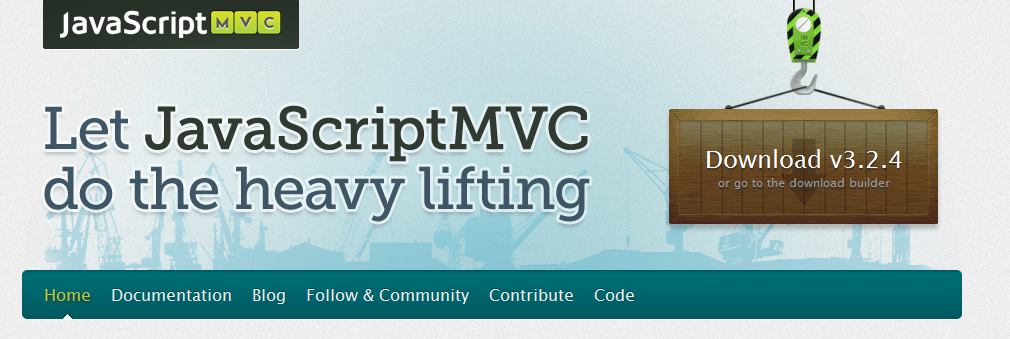
\includegraphics[scale=0.6]{javamvc.png}
			Figure that created by JavaScriptMVC
			\end{center}
		\subsubsection{JQuery}
			\begin{itemize}
				\item Overview: JQuery is free, open source software, licensed under the MIT License. It's also one of the best JavaScript frameworks at presence.
				\item Pros: 
					\begin{itemize}
						\item Easy to use
						\item Large library
						\item Strong community
						\item Great documents and tutorials
						\item Ajax support
					\end{itemize}
				\item Cons:
					\begin{itemize}
						\item Functionality maybe limited
					
					\end{itemize}
			\end{itemize}
			\begin{figure}
				\begin{center}
				\includegraphics[scale=1.2]{jquery.png}
				\caption{An example created by JQuery}
				\end{center}
			
			\end{figure}

		\subsubsection{Cappuccino}
			\begin{itemize}
				\item Overview: an open source framework that makes it easy to build desktop-caliber applications that run in a web browser which look and feel like desktop applications on Mac OS X.
				\item Pros: 
					\begin{itemize}
						\item allow you to create true desktop-like apps right inside the browser
						\item don’t rely on a continous web connection
						\item as fast as desktop app
						\item you can build asyncronous, offline, robust web apps right inside the browser
						\item Cappuccino is compatible with many of the latest browsers
					
					\end{itemize}
				\item Cons:
					\begin{itemize}
						\item Adding a layer of abstraction (Objective-J objects to Javascript) also adds to the overhead. The result is that the application can be slow, particularly if the user's computer is slow.
						\item It is not designed to make full-fledged web sites. That leads to complex and interactive sites may not suitable
						\item is still very early in its development stages, so some parts are still unimplemented
						\item Different Underlying Model
					\end{itemize}
			\end{itemize}
			\begin{figure}
				\begin{center}
				\includegraphics[scale=1.3]{Cappuccino1.png}
				\caption{An example created by cappucino}
				\end{center}
			\end{figure}
		\subsubsection{Ember.js}
			\begin{itemize}
				\item Overview: Ember is a JavaScript framework for creating ambitious web applications that eliminates boilerplate and provides a standard application architecture. Same company with Sproutcore.
				\item Pros: 
					\begin{itemize}
						\item easily implementing MVC functionality.
						\item extremely easy to create computed properties in JavaScript
						\item It is designed so you don't have to worry about whether or not you have 2000 bindings.
						\item is intended for "web-styled" applications.
					\end{itemize}
				\item Cons:
					\begin{itemize}
						\item Documents are not quite clear and understandable.
					
					\end{itemize}
			\end{itemize}
			\begin{figure}
			\begin{center}
			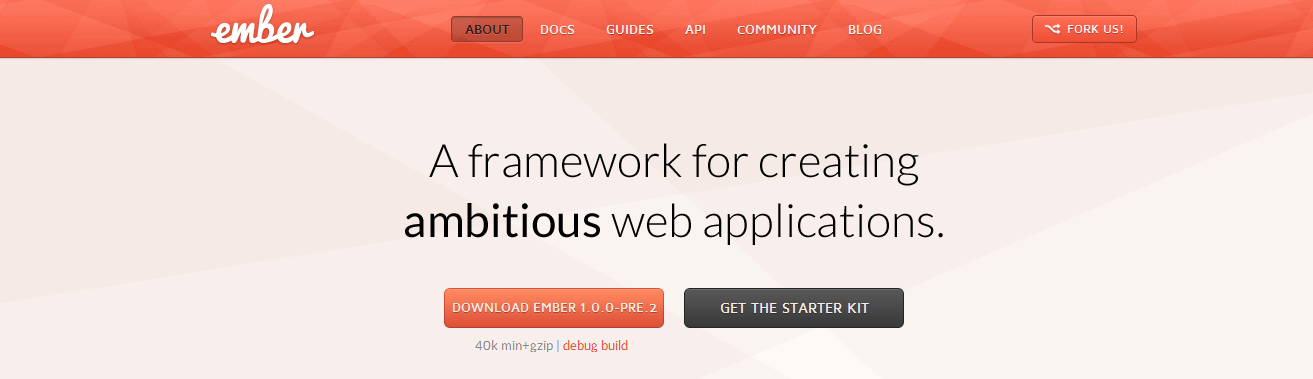
\includegraphics[scale=0.5]{ember.png}
			\caption{An example created by ember}
			\end{center}			
			\end{figure}

		\subsubsection{Flame.js}
			\begin{itemize}
				\item Overview: It's a widget/UI library for Ember.js, so it has all the properties of Ember.js listed above.
				
			\end{itemize}
		\subsubsection{Angular.js}
			\begin{itemize}
				\item Overview:  an open-source JavaScript framework.
				\item Pros: 
					\begin{itemize}
						\item You don't have to write all the event listening and event triggering. Its automatic.
						\item if you want something declarative that uses the View to derive behaviour.
						\item focuses on achieving this through custom HTML tags.
						\item great for small- to intermediate-scale applications
					\end{itemize}
				\item Cons:
					\begin{itemize}
						\item Obtrusively mixes all controller, model and view into the html
						\item invents its own syntax which requires learning
						\item Javascript errors happen if you DON'T clutter the window object.
						\item the more bound elements in your app, the slower it gets
						\item Difficult to allow browsers to optimize this in native code.
						\item It only provides an interface between a combined M, V and C. What if you wanted a Model to subscribe to another Model but didn't want to update a view. You can't do this with Angular.js, but you can with Backbone.
					\end{itemize}
					\begin{figure}
						\begin{center}
							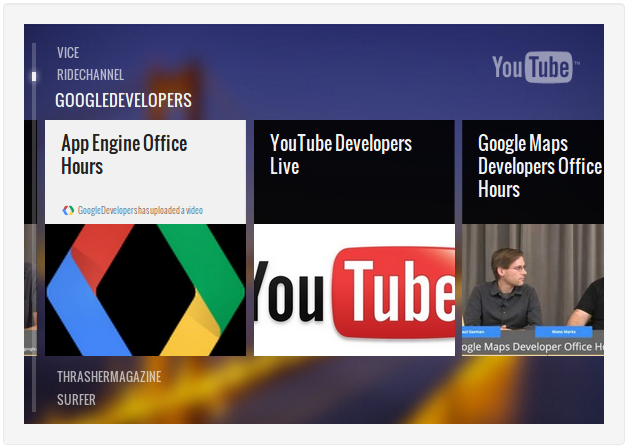
\includegraphics[scale=0.5]{Angular.png}
							\caption{An example created by AngularJS}
						\end{center}
					\end{figure}
			\end{itemize}
		\subsubsection{Twitter Bootstrap}
			\begin{itemize}
				\item Overview:  is a free collection of tools for creating websites and web applications. It contains HTML and CSS-based design templates for typography, forms, buttons, charts, navigation and other interface components, as well as optional JavaScript extensions.
				\item Pros: 
					\begin{itemize}
						\item The framework can be adapted to any CMS or blogging platform like WordPress, Drupal or Joomla.
						\item  Easy visual consistency in your application.
						\item This framework is designed for a web application (not a website) and all the elements fit nicely together to get the app done fast.
						\item many beautiful theme"
						\item Speed, Consistency across applications
						\item People find it simple and elegant"
					\end{itemize}
				\item Cons:
					\begin{itemize}
						\item  incomplete support for HTML5 and CSS 3, but it is compatible with all major browsers.
						\item It uses Less css. but many people like to use other tool to mangage css
					
					\end{itemize}
			\end{itemize}
			\begin{figure}
				\begin{center}
				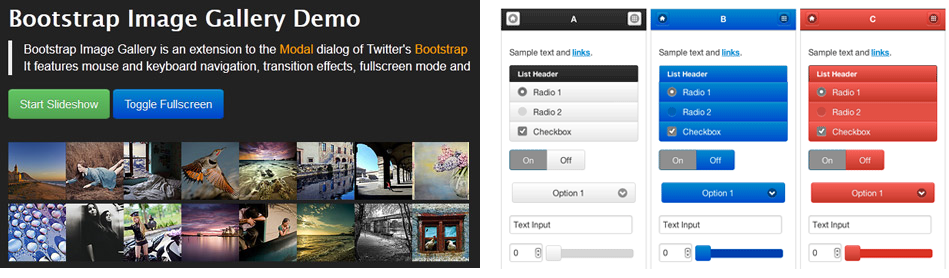
\includegraphics[scale=0.7]{twitter.png}
				\caption{An example that created by Twitter Bootstrap}
				\end{center}				
			\end{figure}

		\subsubsection{Ext JS/Sencha}
			\begin{itemize}
				\item Overview:  a pure JavaScript application framework for building interactive web applications using techniques such as Ajax, DHTML and DOM scripting.
				\item Pros: 
					\begin{itemize}
						\item is like a superset of the widgets like simple label, textbox buttons to complex grids, drag-drop panel
						\item It has quite good documentation with tutorials, samples and user community.
						\item Active and currently most adopted javascript RIA framework
						\item  Good code quality/readability
						\item  Ext JS makes it simple to edit tickets inline
					\end{itemize}
				\item Cons:
					\begin{itemize}
						\item Loading time would is high for home page on web.
						\item CSS – very easy to get lost. It is difficult to find correct class names.
						\item HTML – full of divs and overly complex generated code. Difficult to debug even with FireBug.
						\item  Customization is not easily achievable.
						\item Loading even simple things requires few lines of coding which is simpler in plain html or jQuery
						\item Need quite experienced developer"
					\end{itemize}
			\end{itemize}
			
			\begin{figure}
				\begin{center}
				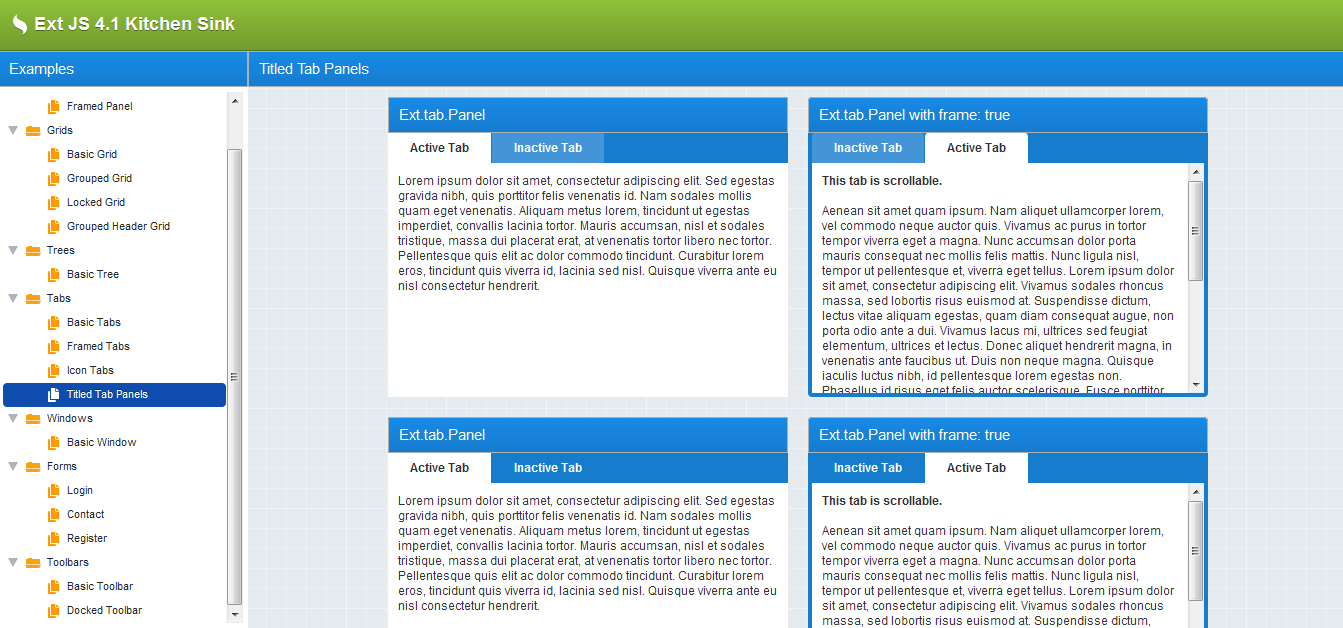
\includegraphics[scale=0.5]{sencha.png}
				\caption{An example that created by sencha}
				\end{center}
			\end{figure}
			
			\begin{figure}
				\begin{center}
				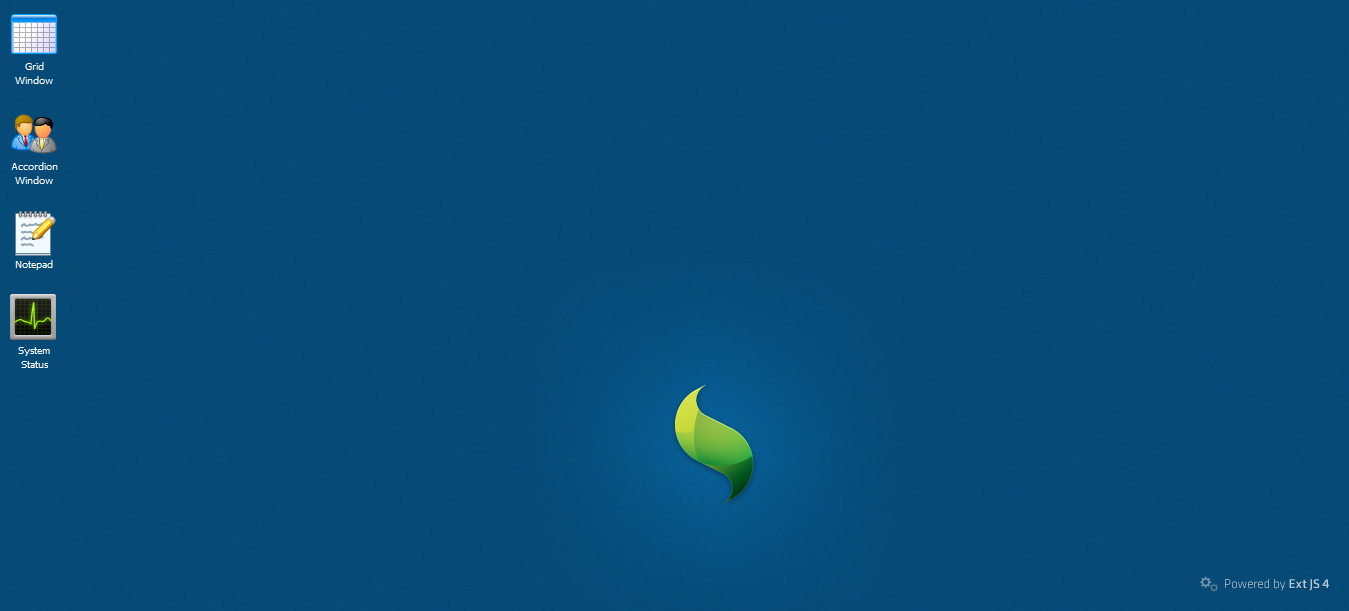
\includegraphics[scale=0.5]{sencha1.png}
				\caption{Another example that created by sencha}
				\end{center}
			\end{figure}					
			
			
		\subsubsection{quooxdoo}
			\begin{itemize}
				\item Overview: ooxdoo is a universal JavaScript framework with a coherent set of individual components and a powerful toolchain
				\item Pros: 
					\begin{itemize}
						\item supports namespace,eventbiding,cross-browser back button, bookmarkability, AOP
						\item feature supports Browser abstraction, DOM manipulation, Events, Templating, Animation.
					\end{itemize}
				\item Cons:
					\begin{itemize}
						\item non CSS -based styling
					
					\end{itemize}
			\end{itemize}
			\begin{figure}
				\begin{center}
				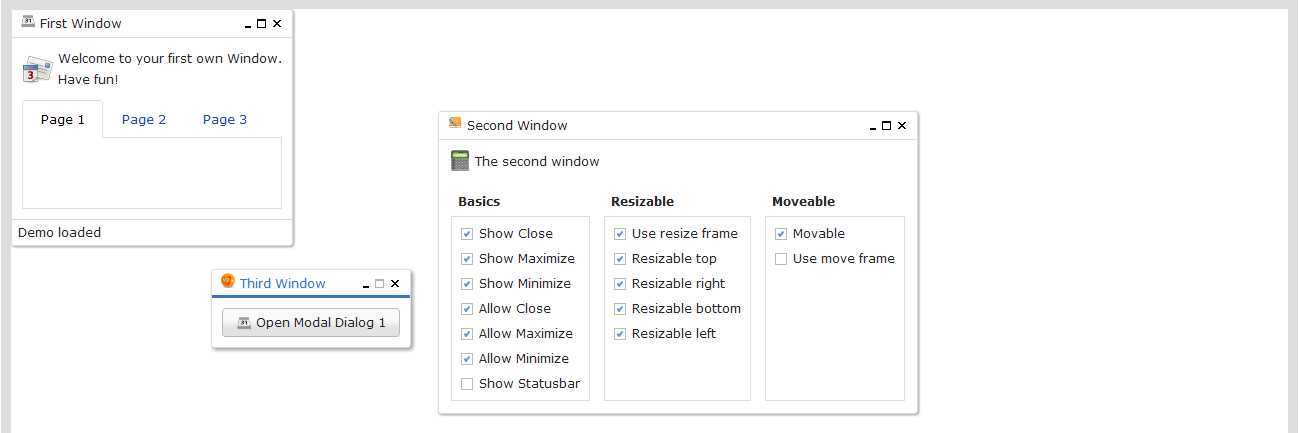
\includegraphics[scale=0.6]{qooxdoo.png}
				\caption{An example that created by qooxdoo}
				\end{center}
			\end{figure}

		\subsubsection{JQueryUI}
			\begin{itemize}
				\item Overview: a curated set of user interface interactions, effects, widgets, and themes built on top of the jQuery JavaScript Library. Whether you're building highly interactive web applications or you just need to add a date picker to a form control, jQuery UI is the perfect choice.
				\item Pros: 
					\begin{itemize}
						\item Base on one of the most popular framework now.
						\item Stable
						\item Nice Theme
						\item support interaction
						\item MIT license
						\item One of the nicest things from jQuery.UI I think is the widget factory, which gives you a quick way of creating your own plug-ins.
						\item is extremely easy to use. Built-in functions are very comprehensive. Compatibility is good.
					\end{itemize}
				\item Cons:
					\begin{itemize}
						\item too heavy
						\item javaScript 's cons
					
					\end{itemize}
			\end{itemize}
			\begin{figure}
				\begin{center}
				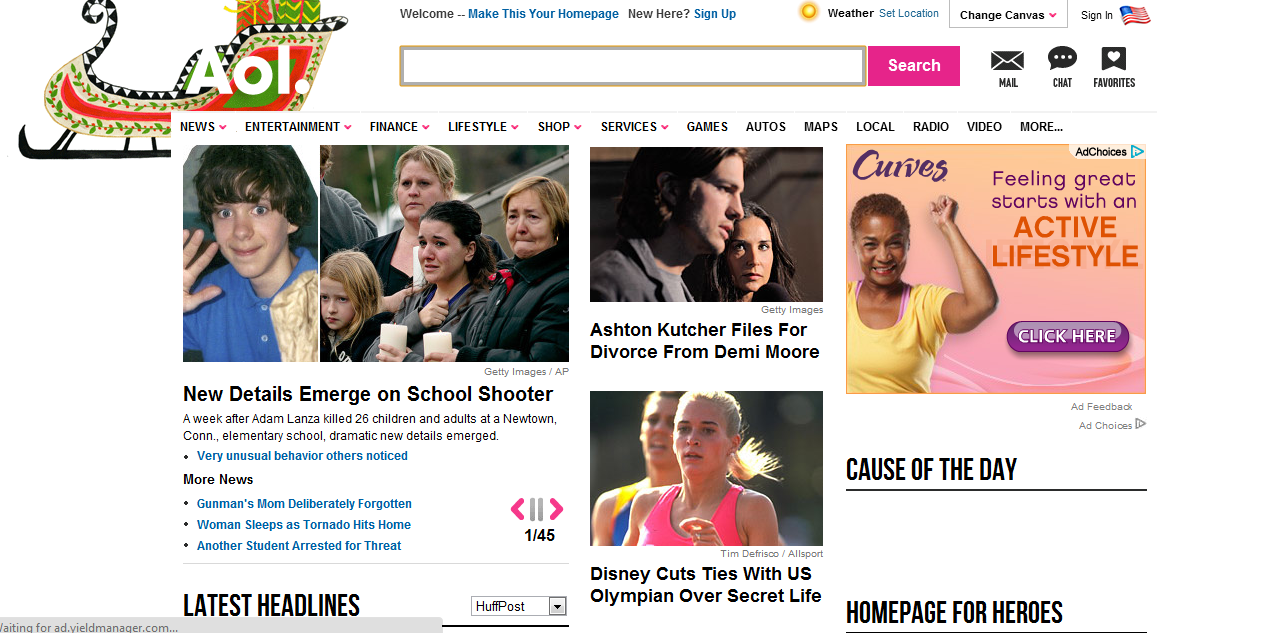
\includegraphics[scale=0.5]{jqueryui.png}
				\caption{An example that created by jqueryui}
				\end{center}
			\end{figure}

		\subsubsection{YUI}
			\begin{itemize}
				\item Overview: an open-source JavaScript library for building richly interactive web applications using techniques such as Ajax, DHTML and DOM scripting.
				\item Pros: 
					\begin{itemize}
						\item support models, views and routers and make it simple to write multi-view applications supporting routing, View transitions and more.
						\item it is a complete solution that includes widgets/components as well as the tools needed to create an organized application architecture.
						\item have scaffolding tools (yuiproject), but these need to be updated
						\item includes all of the goodies of Backbone
					\end{itemize}
				\item Cons:
					\begin{itemize}
						\item it should support some of the auto-wiring (optional) of Ember
						\item should have more AMD-compatible module loader"
					
					\end{itemize}
			\end{itemize}
			\begin{figure}
				\begin{center}
				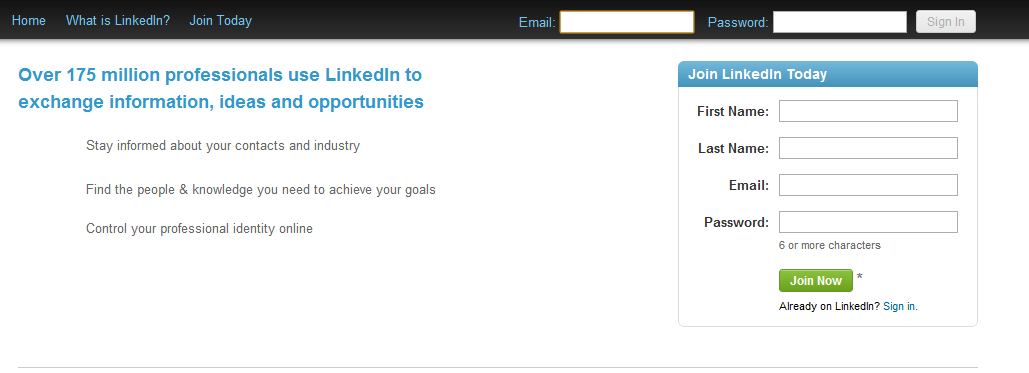
\includegraphics[scale=0.6]{YUI.png}
				\caption{An example that created by YUI}
				\end{center}			
			\end{figure}

			\subsubsection{Backbone.js}
			\begin{itemize}
				\item Overview: Backbone.js gives structure to web applications by providing models with key-value binding and custom events, collections with a rich API of enumerable functions, views with declarative event handling, and connects it all to your existing API over a RESTful JSON interface.
				\item Pros: 
					\begin{itemize}
						\item support a persistence layer and RESTful sync, models, views (with controllers), event-driven communication, templating and routing.
						\item suitable  to build non-trivial applications
						\item quickly depart from one another in how they expect you to approach building apps.
						\item more suitable with something flexible which offers a minimalist solution to separating concerns in my application
						\item you want control, and compatibility with other frameworks.
					\end{itemize}
				\item Cons:
					\begin{itemize}
						\item  A bit clunky, always having to create both the event trigger and event listener in all all view, model, router etc, which makes for larger code and longer figuring it out writing it.
					\end{itemize}
			\end{itemize}
			\begin{figure}
				\begin{center}
				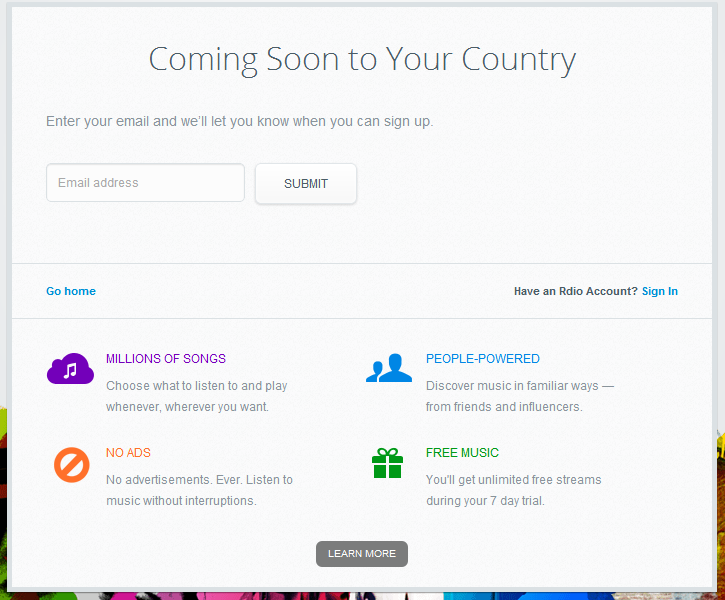
\includegraphics[scale=0.9]{backbone.png}
				\caption{An example that created by backbone}
				\end{center}
			\end{figure}

			\subsubsection{DHTMLX}
			\begin{itemize}
				\item Overview:DHTMLX Touch is an HTML5-based JavaScript library for building mobile web applications. It’s not just a set of UI widgets, but a complete framework that allows you to create eye-catching, cross-platform web applications for mobile and touchscreen devices.
				\item Pros: 
					\begin{itemize}
						\item Great features and UI components.
						\item Great tutorials and samples.
						\item Doesn't conflict with well-known AJAX framework like: JQuery, YUI,..
						\item The library works in all modern browsers: 
						
					\end{itemize}
				\item Cons:
					\begin{itemize}
						\item
					
					\end{itemize}
			\end{itemize}
			\begin{figure}
				\begin{center}
				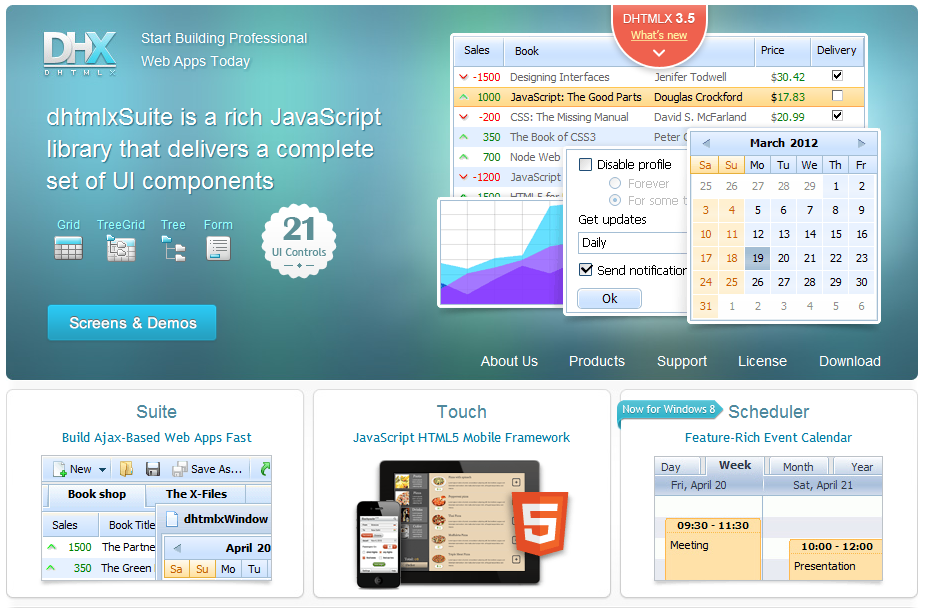
\includegraphics[scale=0.7]{dhtmlx.png}
				\caption{An example that created by DHTMLX}
				\end{center}			
			\end{figure}

			\subsubsection{Rialto}
			\begin{itemize}
				\item Overview: Rialto (Rich Internet Application Toolkit) is a cross browser ajax based JavaScript widgets library. Because it is technology agnostic it can be encapsulated in JSP, JSF, Python, .Net or PHP graphic components.
				\item Pros: 
					\begin{itemize}
						\item is designed for SPA
						\item Widgets library includes: forms, dragdrop, tree, data list with fix header and resizable columns, pop up, splitter.
					\end{itemize}
				\item Cons:
					\begin{itemize}
						\item The documents and demos seem to be vague 
						\item the community is not so active
					
					\end{itemize}
			\end{itemize}
			
The Tables below provide an overview of available MV* frameworks. Columns in the table show the different frameworks, while the  rows classify them with respect to the classification dimensions introduced .The character "x" equals to "yes" and "-" equals to "no". Furthermore additional information for every framework is provided: These following tables show more information about those JavaScript frameworks. The tables also reveal the uniform distribution of MVC and MVVM frameworks as well as JavaScript being the predominant programming language. Furthermore most of the frameworks require no special integration process to be used within an application. Usually it is enough to include a single JavaScript file into the application’s source code. 			
			\begin{table}
				\begin{center}
					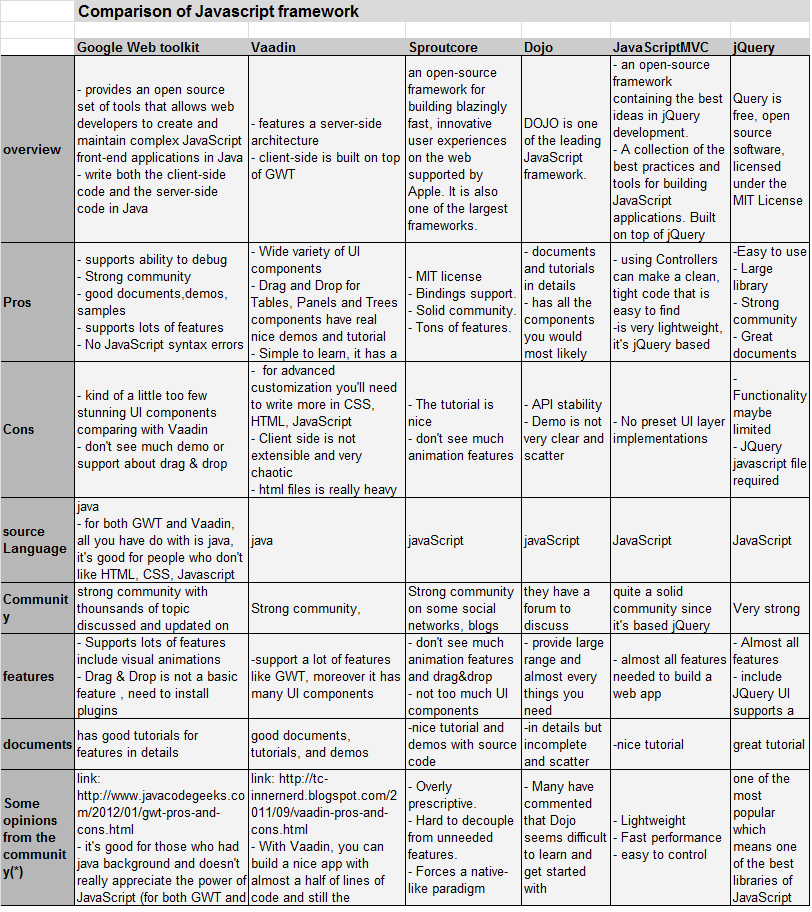
\includegraphics[scale=0.6]{JavaFrameTable1.png}
				
					\caption{Some of JavaScript frameworks in the survey}
				\end{center}
			
			\end{table}
			\begin{table}
				\begin{center}
					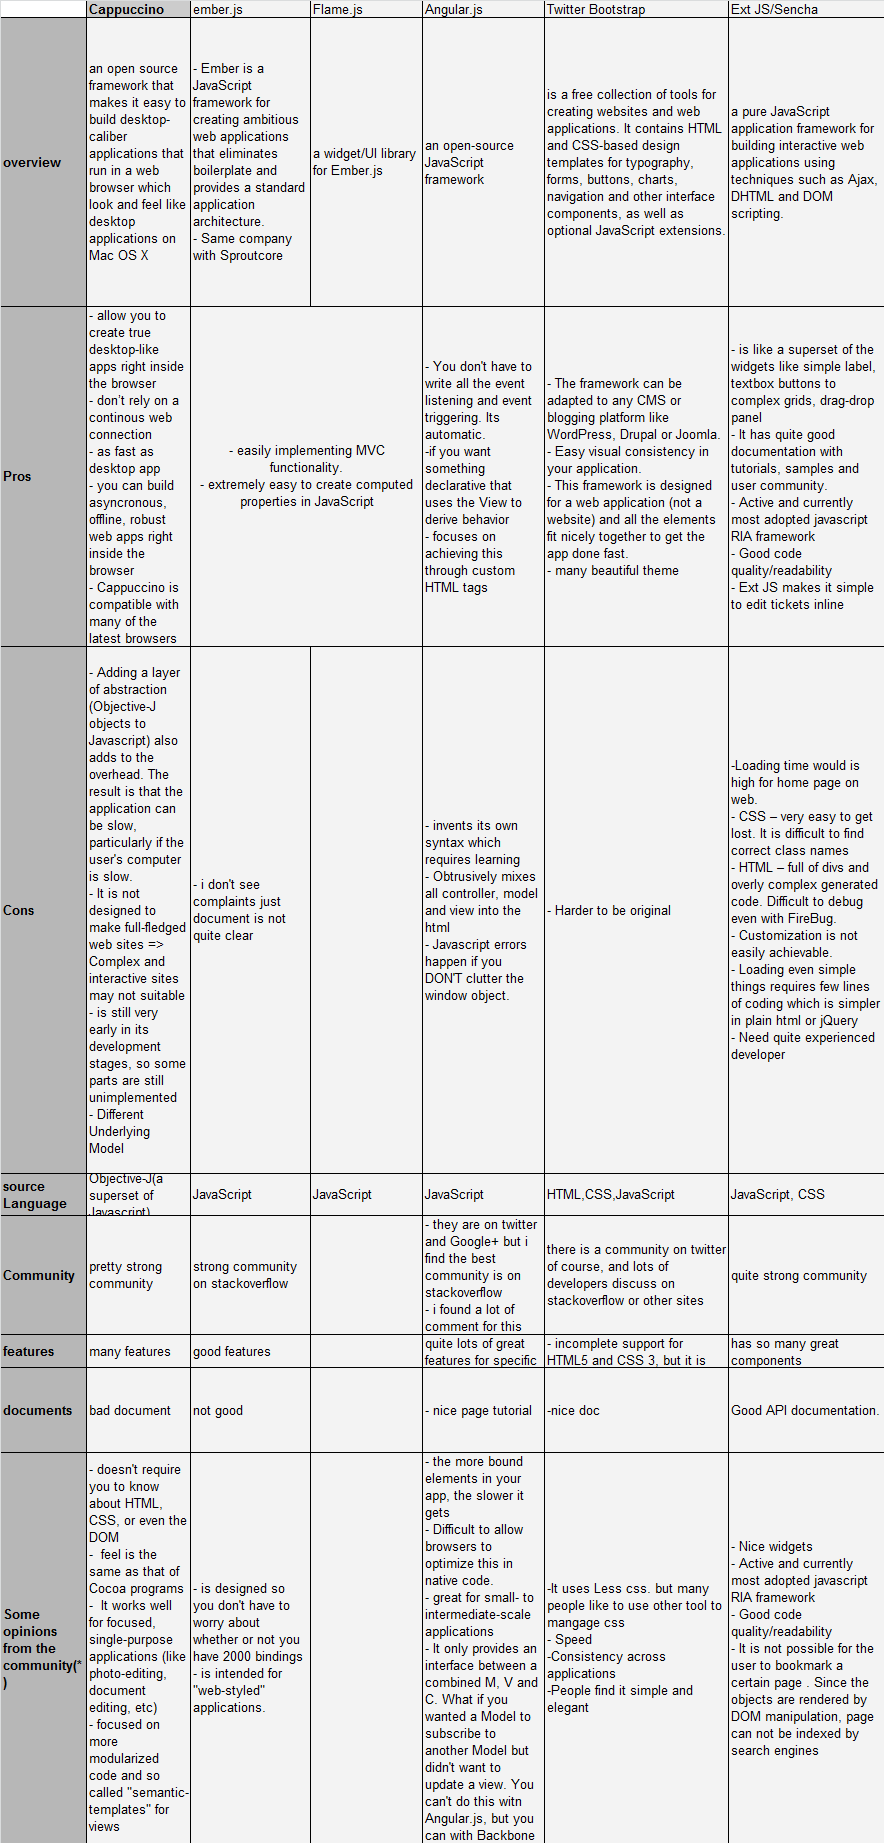
\includegraphics[scale=0.4]{JavaFrameTable2.png}
				
					\caption{Some of JavaScript frameworks in the survey}
				\end{center}
			
			\end{table}
			\begin{table}
				\begin{center}
					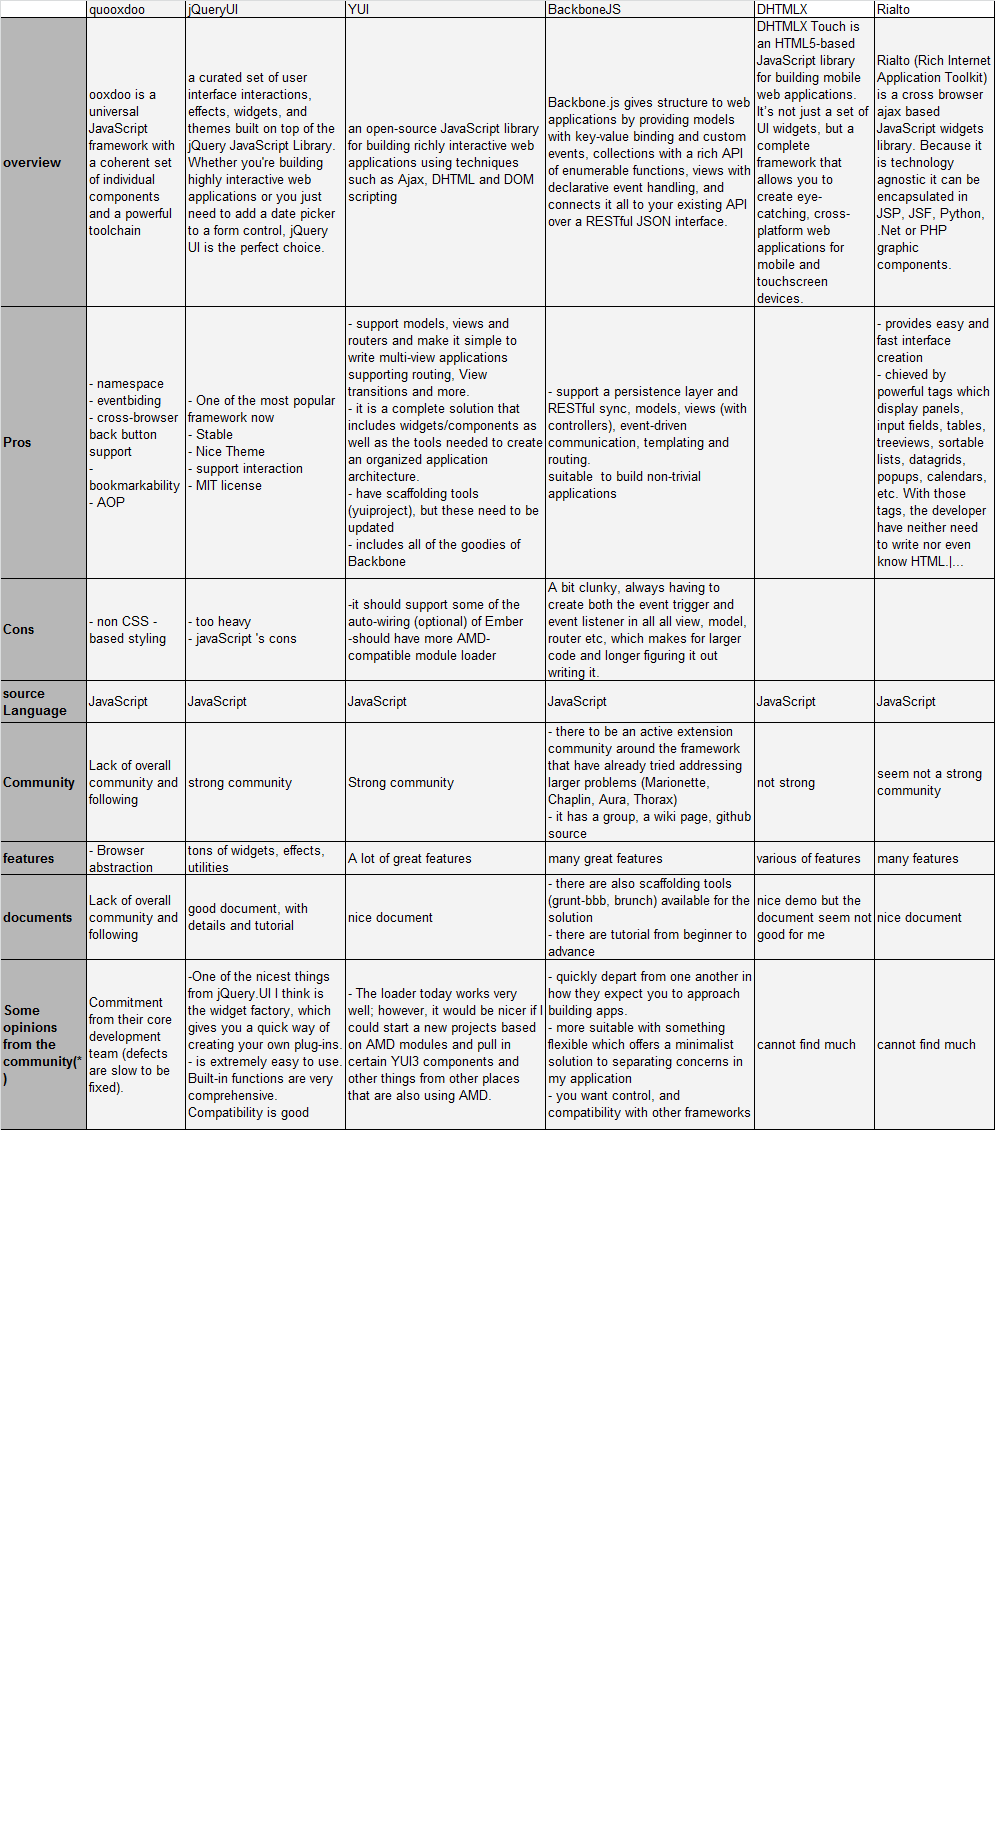
\includegraphics[scale=0.6]{JavaFrameTable3.png}
				
					\caption{Some of JavaScript frameworks in the survey}
				\end{center}
			
			\end{table}
			\begin{table}
				\begin{center}
					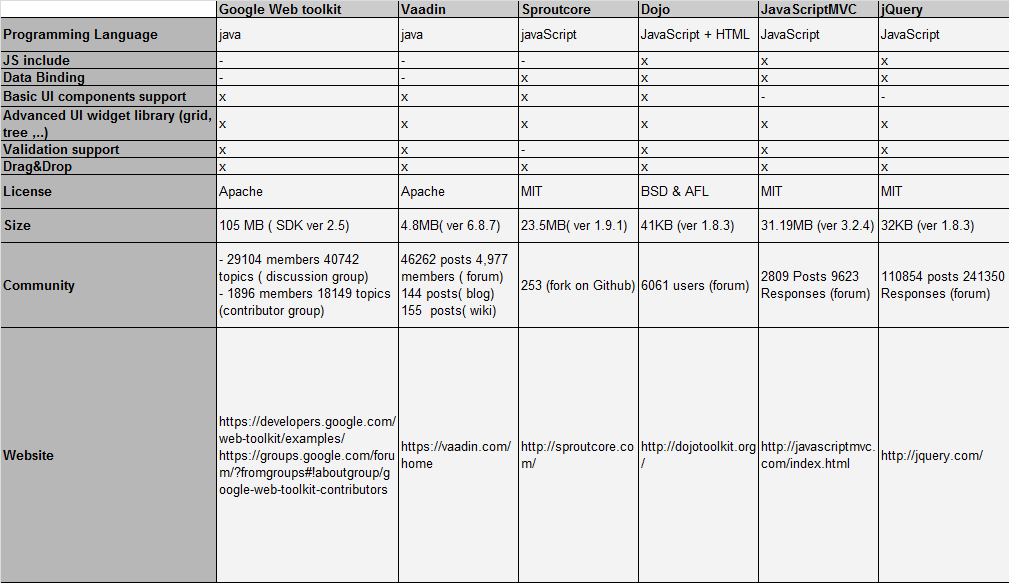
\includegraphics[scale=0.6]{JavaFrameTable1NewCriteria.png}
				
					\caption{Some of JavaScript frameworks in the survey}
				\end{center}
			
			\end{table}
			\begin{table}
				\begin{center}
					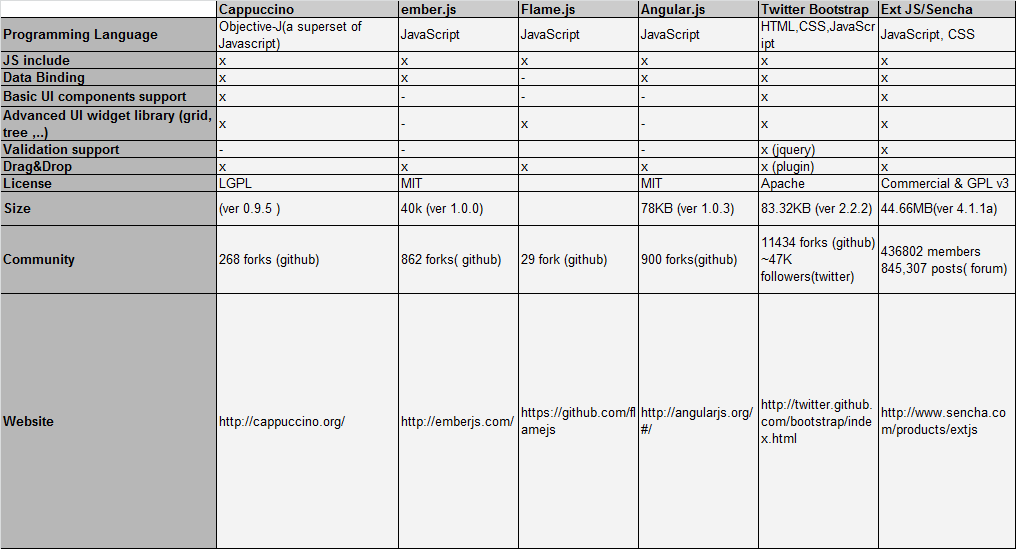
\includegraphics[scale=0.6]{JavaFrameTable2NewCriteria.png}
				
					\caption{Some of JavaScript frameworks in the survey}
				\end{center}
			
			\end{table}
			\begin{table}
				\begin{center}
					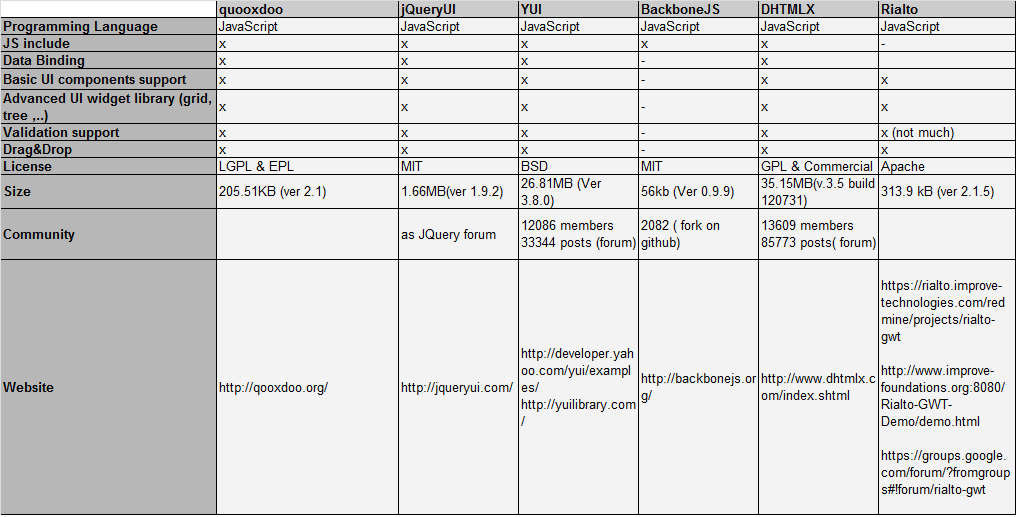
\includegraphics[scale=0.6]{JavaFrameTable3NewCriteria.png}
				
					\caption{Some of JavaScript frameworks in the survey}
				\end{center}
			
			\end{table}


		\subsection{Selected Framework}
			\subsubsection{Angular.js}
		Angular.js is a JavaScript framework released under the open source MIT license. The implementation is based on JavaScript and has a very small footprint (78 kB minified). Since Angular.js has no dependencies it can be used in conjunction with any other JavaScript library. For developers a very comprehensive set of documentation is available comprising an API specification, interactive tutorials as well as running examples. Moreover, Angular.js is special JavaScript framework which is built particularly for software engineering purpose.Angular.js lets you extend HTML vocabulary for your application. The resulting environment is extraordinarily expressive, readable, and quick to develop.Besides, Angular.js is designed from ground up to be testable. It encourages behavior-view separation, comes pre-bundled with mocks, and takes full advantage of dependency injection. It also comes with end-to-end scenario runner which eliminates test flakiness by understanding the inner workings of AngularJS.
					
 	\section{JavaScript Graph Libraries Selection}
 		\subsection{Overview of some javaScript Graph libraries}
		\subsection{JavaScript Graph Libraries Selection Characteristics} 		
		\subsection{Survey of Existing graph libraries }
		\subsection{Selected graph library}	

\chapter{EXPLORATION OF KEY TECHNOLOGIES}
\textsl{In this chapter, I will present all the key technologies that i have been using in this thesis. For each technology, a brief overview will be introduced as well as their main features, advantages. Some important concept are also presented}

	\section{AngularJS}
		\subsection{overview}
		AngularJS is a structural framework for dynamic web apps. It lets you use HTML as your template language and lets you extend HTML's syntax to express your application's components clearly and succinctly. Out of the box, it eliminates much of the code you currently write through data binding and dependency injection. And it all happens in JavaScript within the browser, making it an ideal partner with any server technology.

Angular is what HTML would have been had it been designed for applications. HTML is a great declarative language for static documents. It does not contain much in the way of creating applications, and as a result building web applications is an exercise in what do I have to do to trick the browser into doing what I want.

The impedance mismatch between dynamic applications and static documents is often solved with:
\begin{itemize}
\item a library - a collection of functions which are useful when writing web apps. Your code is in charge and it calls into the library when it sees fit. E.g., jQuery.
\item frameworks - a particular implementation of a web application, where your code fills in the details. The framework is in charge and it calls into your code when it needs something app specific. E.g., knockout, ember, etc.

\end{itemize}


Angular takes another approach. It attempts to minimize the impedance mismatch between document centric HTML and what an application needs by creating new HTML constructs. Angular teaches the browser new syntax through a construct we call directives. Examples include:

\begin{itemize}
\item Data binding, as in {{}}.
\item DOM control structures for repeating/hiding DOM fragments.
\item Support for forms and form validation.
\item Attaching code-behind to DOM elements.
\item Grouping of HTML into reusable components.

\end{itemize}
		
		\subsection{Why Angular?}
			
		\subsection{Dependency Injection}
			\subsubsection{Introduction}
			There are only three ways an object or a function can get a hold of its dependencies:
\begin{enumerate}
\item The dependency can be created, typically using the new operator or asking a factory object to make one.
\begin{verbatim}
public SomeClass() {

 myObject = new Object(objectname);

}

public SomeClass() {

 myObject = Factory.getObject(objectname);

}
\end{verbatim}
\item The dependency can be looked up by referring to a global variable.
\begin{verbatim}
public SomeClass() {

 myObject = GLOBAL_OBJECT;

}
\end{verbatim}
\item The dependency can be passed in to where it is needed.
\begin{verbatim}
public SomeClass (Object myObject) {

 this.myObject = myObject;

}
\end{verbatim}

\end{enumerate}

The first two option are quite bad. Hardcoding the \emph{objectname} does not really solve the problem as you cannot easily change your mind later without changing the that class again. Using a constant \emph{GLOBAL\_OBJECT} is also a bad idea as the \emph{SomeClass} now depends on a constant to be set.
\\

But there is yet another problem that cannot be solved easily: How can I change Object class? For instance, to replace it with a mock object to ease testing. This makes the class difficult to modify the dependencies. This is especially problematic in tests, again ,where it is often desirable to provide mock dependencies for test isolation[].
\\

The third option , which simply passed the dependencies into where it is needed , is the 

most viable, since it removes the responsibility of locating the dependency from the component. The dependency is simply handed to the component.That's Dependency Injection. Nothing more! Using the SomeClass class is now a bit more 
involving as you first need to create the object:
\begin{verbatim}
myObject = new Object(objectname);

someInstance = new SomeClass(myObject);
\end{verbatim}
Basically, DI can be simply explained as follow, instead of having the objects creating a dependency or asking a factory object to make one for them, you pass the needed dependencies in to the constructor, and you make it somebody else's problems . One of the major advantages of dependency injection is that it can make testing lots easier. 
\\

This is just for your first sight of what will happen to the code and how it looks like when we use DI. I’ll explain why we are doing this and its benefits later. First, let’s see what is the definition of this design pattern.

			\subsubsection{Definition}
			Dependency injection (DI) is a software design pattern that allows removing hard-coded dependencies and making it possible to change them, whether at run-time or compile-time[1]

Dependency injection involves at least three elements:
\begin{itemize}
\item a dependent consumer,
\item a declaration of a component's dependencies, defined as interface contracts,
\item an injector (sometimes referred to as a provider or container) that creates instances of classes that implement a given dependency interface on request.
\end{itemize}

The dependent object describes what component it depends on to do its work. The injector decides what concrete classes satisfy the requirements of the dependent object, and provides them to the dependent.
\\

Being able to make this decision at run-time rather than compile time is the key advantage of dependency injection. Multiple, different implementations of a single software component can be created at run-time and passed (injected) into the same test code. The test code can then test each different software component without 
being aware that what has been injected is implemented differently.
			\subsubsection{Types}
			Dependency Injection is not restricted to constructor injection:

\begin{itemize}
\item Constructor injection
\begin{verbatim}
public SomeClass {

SomeClass(myObject)

{

 this.myObject = myObject;

}

}


\end{verbatim}
\item Setter Injection:
\begin{verbatim}


public SomeClass {

public Setter(myObject)

{

 this.myObject = myObject;

}

}
\end{verbatim}
\item  Property Injection:
\begin{verbatim}


public SomeClass {

public ObjectProperty;

}

someClass->ObjectProperty = property;
\end{verbatim}
\end{itemize}
		\subsubsection{Benefits}
\begin{itemize}
\item Reduction of boilerplate code – which is included in many places without any alteration and the programmers have to write more code to do minimum jobs in the application objects since all work to initialize or set up dependencies is handled by a provider component . 
\item Very useful when we have objects whose implementations change often 
\item Very useful for large projects where there is issue of maintainability, simplicity.

\item Useful in unit testing, as it is easy to inject a fake implementation of a service into the object being tested by changing the configuration file, or overriding component registrations at run-time.

\item Dependency Injection facilitates the writing of testable code.
\end{itemize}
			\subsubsection{Examples and explanation in AngularJS}
			\begin{verse}
			function SomeClass(greeter) {

this.greeter = greeter;

}

 SomeClass.prototype.doSomething = function(name) {

this.greeter.greet(name);

}
\end{verse}
In the above example SomeClass is not concerned with locating the greeter dependency, it is 

simply handed the greeter at runtime.

This is desirable, but it puts the responsibility of getting hold of the dependency on the code that 

constructs SomeClass.

To manage the responsibility of dependency creation, each Angular application has an injector. 

The injector is a service locator that is responsible for construction and lookup of dependencies.
\begin{verse}


1. // Provide the wiring information in a module

2. angular.module('myModule', []).

3. 

4. // Teach the injector how to build a 'greeter'

5. // Notice that greeter itself is dependent on '\$window'

6. factory('greeter', function(\$window) {

7. // This is a factory function, and is responsible for 

8. // creating the 'greet' service.

9. return {

10. greet: function(text) {

11. \$window.alert(text);

12. }

13. };

14. });

15. 

16. // New injector is created from the module. 

17. // (This is usually done automatically by angular bootstrap)

18. var injector = angular.injector(['myModule', 'ng']);

19. 

20. // Request any dependency from the injector

21. var greeter = injector.get('greeter');
			\end{verse}

		\subsection{Separation of Concern}
		\subsection{Inversion of Control}

			
		\subsection{Angular 's key features}
			\subsubsection{Directives}
			\subsubsection{Two-way DataBinding}
			\subsubsection{Filters}
			\subsubsection{MVC}
			\subsubsection{Service vs Factory vs provider}
			\subsubsection{Testing}
	\section{GoJS}
		\subsection{Overview}
		\subsection{Why Gojs?}
		\subsection{Features}
			\subsubsection{drag-and-drop}
			\subsubsection{transactional state and undo management}
			\subsubsection{palettes and	 overviews}
			\subsubsection{data-bound models}
			\subsubsection{event handlers and an extensible tool system for custom operations}
	\section{Mongodb}
		\subsection{Overview}
		\subsection{Why Mongodb?}
		\subsection{Introduction to MongoLab}
	\section{Angular Bootstrap}
	\section{Jquery}
	\section{Semantic-UI}
	\section{HTML5}
	\section{CSS3}
\chapter{BUILDING AN APPLICATION USING SELECTED TECHNOLOGIES}
	

	

\chapter{DISCUSSION \& CONCLUSION}

\begin{thebibliography}{99}
\bibitem{survey}{ "Surveying the digital future" UCLA Internet Report, http://www.digitalcenter.org/pdf/InternetReportYearThree.pdf}

\bibitem{Gvu} {“Gvu 10th www user survey,” GVU, http://www.cc.gatech.edu/gvu/user\_surveys/survey-1998-10/}

\bibitem{Center} “Center for the digital future: 2008 digital future report,” 2009. University of Southern California (USC) Annenberg School, C.F.T.D.F.

\bibitem{Internet} {L. Rainee, “Internet, broadband and cellphone statistics,” 2010. http://www.pewinternet.org/Reports/2010/Internet-broadband-and-cell-phone-statistics.aspx.}

\bibitem{Online} P. R. Center, “Online activities,” http://www.pewinternet.org/StaticPages/Trend-Data/Online-Activites-Total.aspx.

\bibitem{RIA} "Rich Internet application " http://en.wikipedia.org/wiki/Rich\_Internet\_application

\bibitem{WebApp} "Web Application" http://en.wikipedia.org/wiki/Web\_application

\bibitem{Real} Franz Josef Grüneberger , "REAL-TIME COLLABORATION SUPPORT FOR JAVASCRIPT FRAMEWORKS"

\bibitem{MT08} Tommi Mikkonen and Antero Taivalsaari. Web Applications Spaghetti Code for the 21st Century. In SERA, pages 319–328, 2008.

\bibitem{Ree79b} Trygve M. H. Reenskaug. Models - Views - Controllers. http://heim.ifi.uio.
no/~trygver/1979/mvc-2/1979-12-MVC.pdf, December 1979.

\bibitem{Ree79a} Trygve M. H. Reenskaug. Thing-Model-View-Editor - an Example from a Planningsys-tem. http://heim.ifi.uio.no/~trygver/1979/mvc-1/1979-05-MVC.
pdf, 1979.

\bibitem{BL12} Tim Berners-Lee. WorldWideWeb, the first Web Client. http://www.w3.org/People/Berners-Lee/WorldWideWeb.html, 2012.

\bibitem{TM11}Antero Taivalsaari and Tommi Mikkonen. The Web as an Application Platform: The Saga Continues. In EUROMICRO-SEAA, pages 170–174, 2011.

\bibitem{Gar05} Jesse James Garrett. AJAX: A New Approach to Web Applications. http://www.adaptivepath.com/ideas/ajax-new-approach-web-applications, 2005.
\end{thebibliography}



\end{document}
